% !TeX spellcheck = en_US
\addsection{AI Heroes}{\spells/fortune.png}

\begin{multicols}{2}

\subsection*{AI Hero Turn}

\textbf{AI Heroes} always start in their Town's Field unless otherwise stated.
They have 3 MP and always use them to perform the following Actions in decreasing priority:
\begin{itemize}
  \item Check if a player's Hero is on the same Tile as the AI.
    If they are, spend all MP to move towards them in an attempt to begin Combat.
  \item Check if there are any Mines or Settlements to Flag on the Map Tile the AI Hero is on.
    If there are any, move toward the closest one and Flag it.
  \item Otherwise, move toward the player's Town in an attempt to Flag it.
Repeat this sequence until all MP is used.
\end{itemize}

\begin{center}
  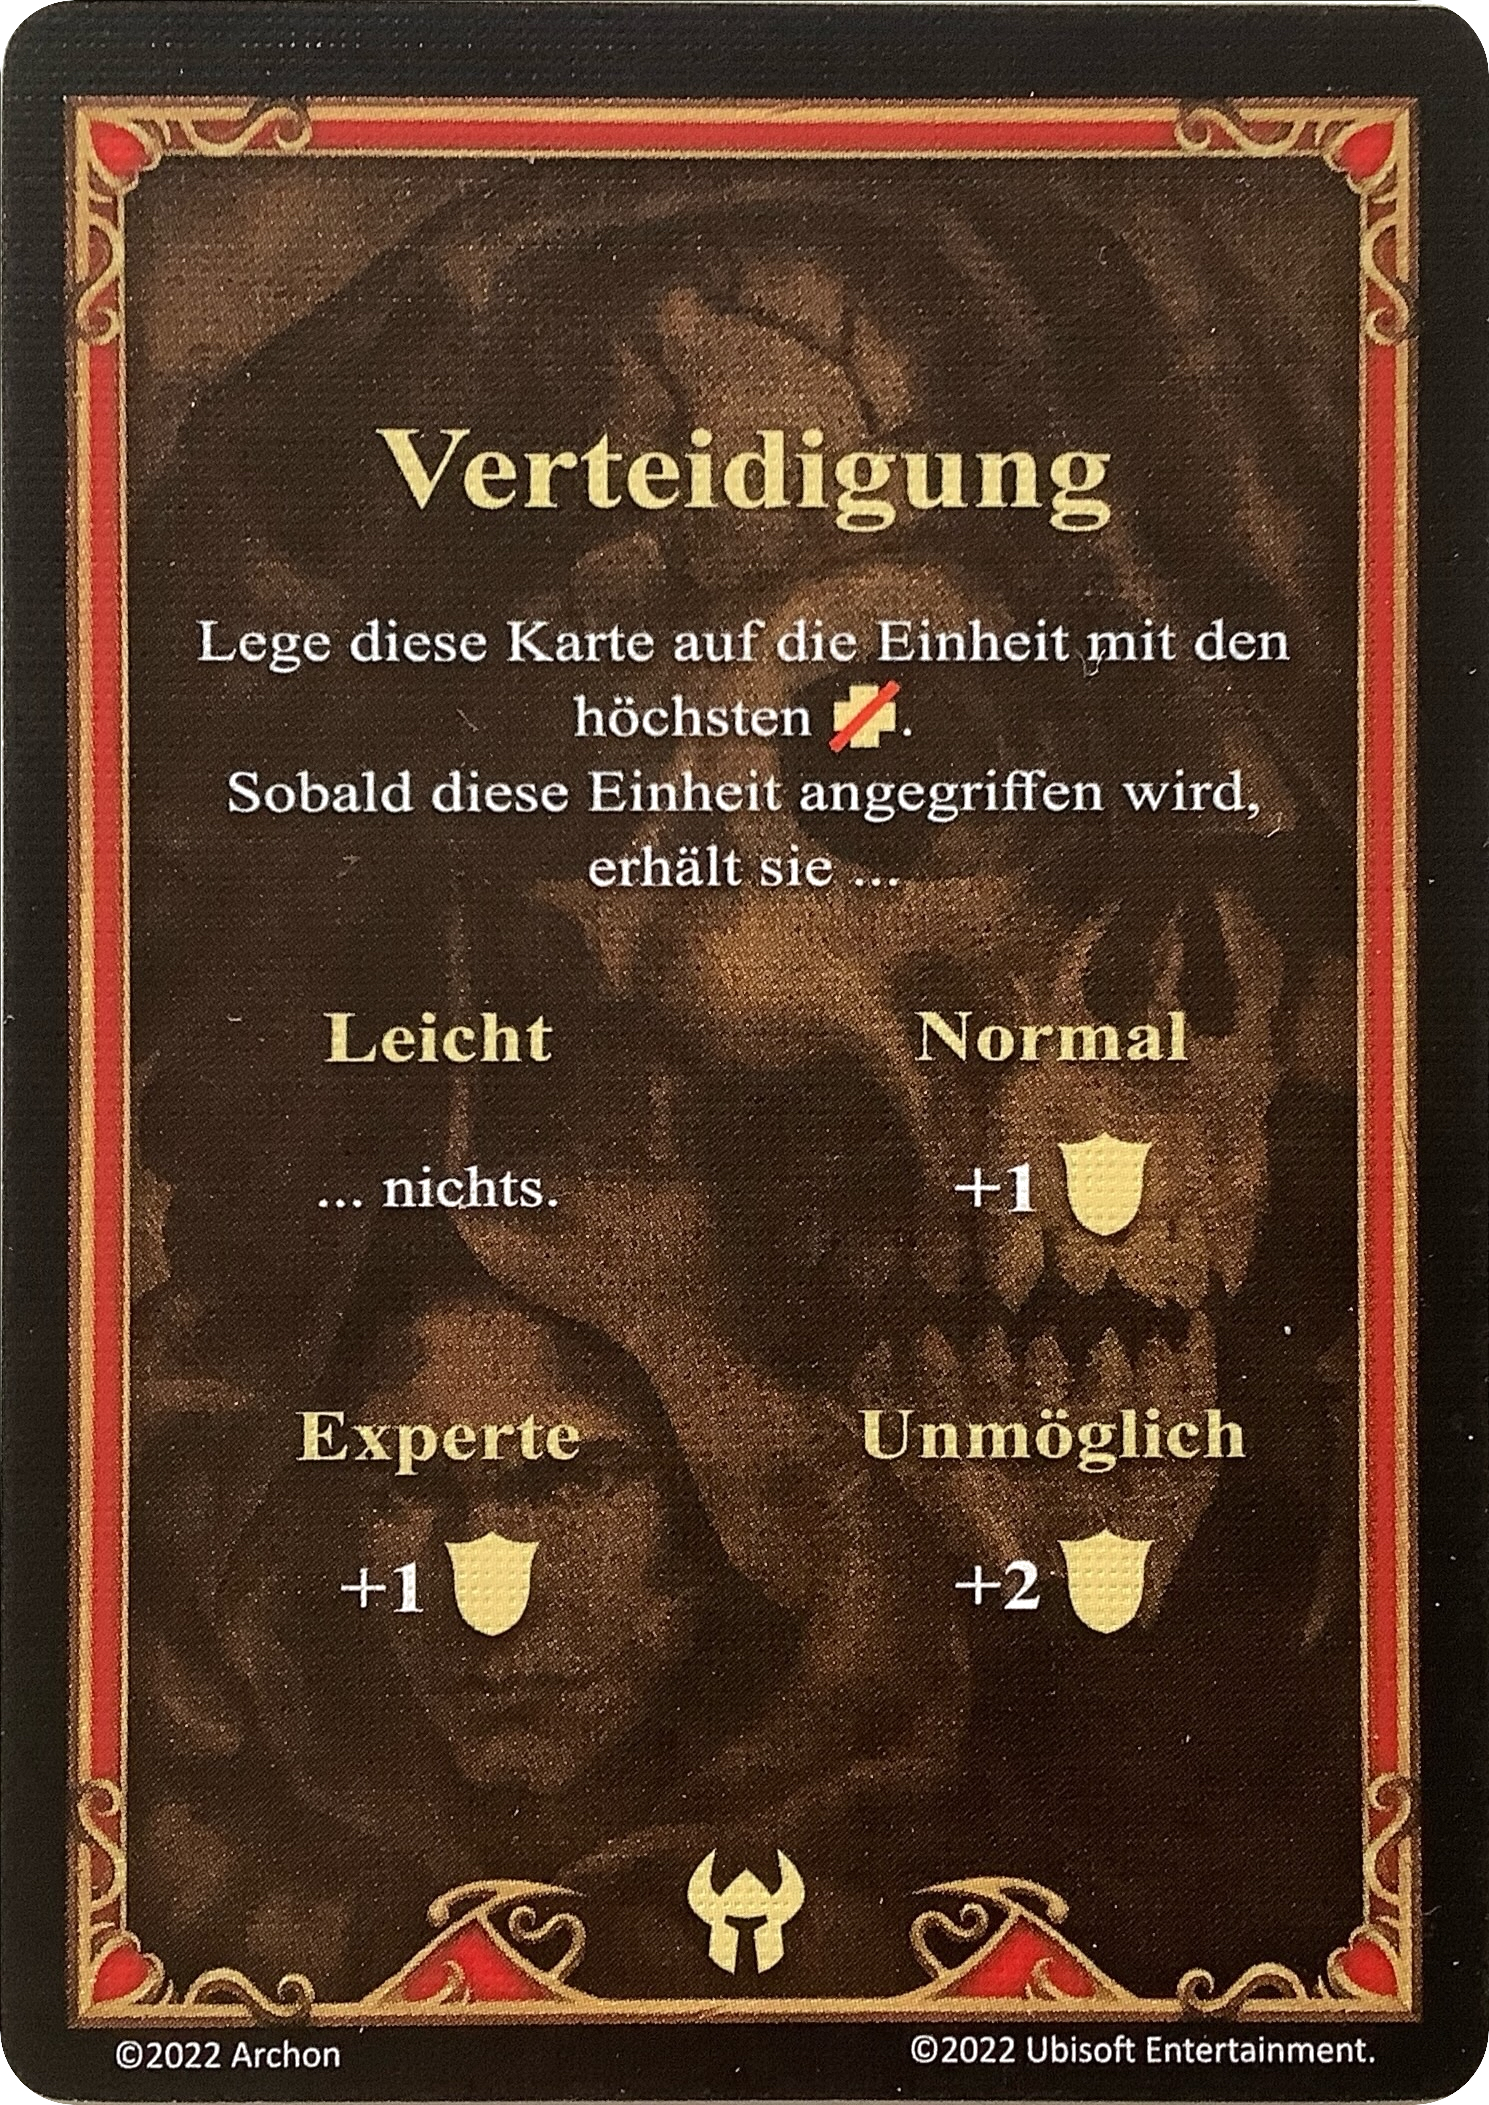
\includegraphics[width=\linewidth]{\cards/ai.png}
\end{center}

AI Heroes always \textbf{automatically win Combat} against any Neutral Units, while simultaneously \textbf{Flagging or Visiting all Fields} they happen to move through.
They gain no benefits from Flagging or Visiting Fields.

AI Heroes must discover face down Map Tiles as normal by spending 1 MP before moving onto them.
The player chooses that tile's orientation.\par
AI Heroes cannot Surrender and you cannot Surrender to them;
they will always fight until they run out of Units.
Winning Combat against an AI Hero does not grant any rewards unless stated by the Scenario.
AI Heroes do not have a Town Board, Resources, or a Hero Card.
Their Units are static and defined by the Scenario's setup or other rules.\par
Any differences to the above will be described in any given Scenario's own rules.

\vfill
\hspace{3em}
\includegraphics[width=\linewidth]{\art/sorrow.png}

\includegraphics[width=\linewidth]{\art/titan.jpg}

\subsection*{\hypertarget{AIrules}{Player vs AI}}

These rules apply when playing a \textbf{Solo} game.\index{Solo Mode}
The AI Combat rules for unit behaviour are also used when playing a \textbf{Cooperative} Scenario.\par
Solo Campaigns are played against AI Heroes who use two automated Decks to play the game: the \textbf{AI Deck}, and the \textbf{Spell Deck}.
Each Campaign Scenario contains instructions for constructing these Decks.\par
The AI Deck consists of cards that are similar in function to Abilities and Artifacts, but change depending on the game's \hyperlink{Difficulty}{Difficulty}.
When an \textbf{AI hero} Activates a Unit, draw an AI Card\index{AI Card} and follow its instructions before the Unit moves and/or attacks.
The Spell Deck should be used when instructed by the cards in the AI Deck.
If an AI Hero is instructed to draw a card, they will draw and resolve another card from the AI Deck.\par

\subsection*{\hypertarget{AI Combat}{Combat against AI}}

During Combat against Neutral enemies or AI Heroes, their Units follow an automatic set of instructions:
\par
\textbf{Initiative rules} work identically.
\includesvg[height=10px]{\svgs/unit_ground.svg} and \includesvg[height=10px]{\svgs/unit_flying.svg} Units prioritize attacking Units of the same tier.
If this is impossible, they attack the closest Unit, prioritizing the lowest tier one.
\includesvg[height=10px]{\svgs/unit_ranged.svg} Units prioritize attacking other \includesvg[height=10px]{\svgs/unit_ranged.svg} Units of the same tier, then lower tier, and finally higher tier.
If there are no \includesvg[height=10px]{\svgs/unit_ranged.svg} Units for them to target they prioritize \includesvg[height=10px]{\svgs/unit_ground.svg} and \includesvg[height=10px]{\svgs/unit_flying.svg} Units in the same tier order.
If there's more than one valid target, they attack the closest one.\par
If there's ever a tie between equally valid targets for any Units, the player chooses which Unit is attacked.
Enemy units cannot \hyperlink{Defend}{Defend} unless instructed to.

\end{multicols}
